% !TEX root = ../../../main.tex
% 来源：高中物理甲种本·第三册（电磁·光学·近代物理）
% 章节：电磁感应 / 楞次定律的应用
% 原始文件：2.tex，行 209-225
% 类型：tikz
% ---
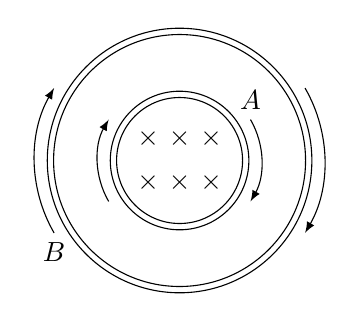
\begin{tikzpicture}[>=latex,scale=.8]
\draw (0,0) circle (1);
\draw (0,0) circle (1.1);
\draw (0,0) circle (2);
\draw (0,0) circle (2.1);
\foreach \x in {-.5, 0, .5}
\foreach \y in {-.35,.35}
{
   \node at (\x,\y){$\times$};
}

\draw[->] (30:1.3) node [above]{$A$} arc (30:-30:1.3);
\draw[->] (30:2.3) arc (30:-30:2.3);
\draw[->] (210:1.3) arc (210:150:1.3);
\draw[->] (210:2.3) node [below]{$B$} arc (210:150:2.3) ;

\end{tikzpicture}
